\batchmode
\documentclass{beamer}
\usepackage[utf8]{inputenc}
\usepackage[ngerman]{babel}

\usetheme[deutsch]{KIT}
\author{Jan Haag (jan.haag@student.kit.edu)}
\title{Programmieren Tutorium 2 -- Datentypen, Werte, Konstruktoren, Methoden}
\institute{Institut f\"{u}r Zeritfizierbare und Vertrauensw\"{u}rdige Informatiksysteme (ZVI)}
\TitleImage[scale=0.225]{frontpic.jpg}

\begin{document}
\begin{frame}
\maketitle
\end{frame}

\begin{frame}
\frametitle{Inhalt}
\tableofcontents
\end{frame}

\section{Datentypen und Werte}
\begin{frame}%[fragile]
\frametitle{Datentypen und ihre Wertebereiche}
\begin{tabular}{lll}
Typ & Kleinster Wert & Gr"o"ster Wert\\
\hline
char & Unicode NULL ($0$) & Unicode \textbackslash{}uFFFF ($65 535$) \\
byte & $-128$ & $127$ \\
short & $-32.768$ & $32.767$ \\
int & $-2.147.483.648$ & $2.147.483.647$ \\
long & $-9.223.372.036.854.775.808$ & $9.223.372.036.854.775.807$\\
float & $-3.4028235\cdot{}10^{38}$ & $3.4028235\cdot{}10^{38}$\\
double & $-1.7976931348623157\cdot{}10^{308}$ & $1.7976931348623157\cdot{}10^{308}$\\
\end{tabular}
\end{frame}

\section{Konstruktoren und Methoden}
\begin{frame}[fragile]
\frametitle{Konstruktoren und Methoden -- Beispiel}
\begin{verbatim}
class Point {
    int x;
    int y;

    public Point(int x, int y) {
        setX(x);
        setY(y);
    }

    int getX() {
        return x;
    }

    int getY() { return y; }
\end{verbatim}
\end{frame}

\begin{frame}[fragile]
\frametitle{Konstruktoren und Methoden -- Beispiel}
\begin{verbatim}
    void setX(int x) {
        this.x = x;
    }

    void setY(int y) {
        this.y = y
    }

    public static void main(String[] args) {
        Point p = new Point(3, 5);
        System.out.println("Point: " + p.getX() + " " + p.getY());
    }
}
\end{verbatim}
\end{frame}

\section{Aufgaben}
\begin{frame}[fragile]
\frametitle{Theorie...}
Werte folgende Ausdr\"{u}cke aus.
\begin{verbatim}
char c = 'a';
int java = 0xcafebabe;

char result = c + 3;
int result = 0xffff & java;
int result = 0xffff | java;
int result = ~0xffff;
int result = java >> 4;
\end{verbatim}
\end{frame}

\begin{frame}
\frametitle{Modellierung eines Autos}
F"uge dem Auto-Modell aus dem letzten Tutorium geeignete Konstruktoren und Methoden hinzu.
\end{frame}

\begin{frame}
\frametitle{Ende}
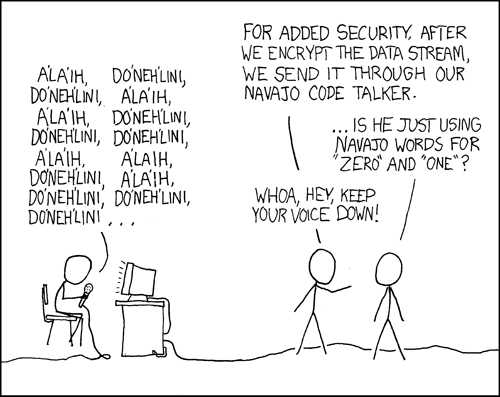
\includegraphics[scale=0.4]{code_talkers.jpg}
\end{frame}
\end{document}
